\chapter{Síntese das perspectivas teóricas}
\label{sinteses}

 O escopo deste capítulo abrangerá o estudo feito sobre os objetos de análise referidos na
 \autoref{sec:ObjetosDeAnalise}, apresentando a síntese das perspectivas abordadas na \autoref{perspectivas}
 da fundamentação teórica com o intuito de esclarecer os pontos chaves presentes em cada arquitetura.
 Para tal, organizou-se os temas discutidos na fundamentação teórica no modelo do \autoref{modelo-sintese} 
apresentado na seção metodológica.

\section{Síntese da arquitetura monolítica}
\label{monoSintese}

\begin{quadro}
    \caption{Arquitetura monolítica - síntese sobre o domínio do problema\label{monolitico:sintese-dominio}}
    \begin{tabularx}{\linewidth}{ | p{5cm} | X | }
    \hline
    \textbf{A escolha de uma}       & arquitetura monolítica \\ \hline
    \textbf{sob a perspectiva}      & da problemática a ser resolvida \\ \hline
    \textbf{mediante o aspecto}     & de domínio sobre o problema \\ \hline
    \textbf{gera um impacto}        & positivo se o domínio sobre o contexto é baixo\\ \hline
    \textbf{devido à }              & arquitetura simplista \\ \hline
    % \textbf{contudo}                & \\ \hline
    % \textbf{consciente de que este aspecto tende a }          & \\ \hline
    \textbf{com base na}            & \autoref{Perspectivas:Problematica} \\ \hline
    \end{tabularx}
\end{quadro}

\begin{quadro}
    \caption{Arquitetura monolítica - síntese sobre o tamanho da aplicação\label{monolitico:sintese-tamanho}}
    \begin{tabularx}{\linewidth}{ | p{5cm} | X | }
    \hline
    \textbf{A escolha de uma}       & arquitetura monolítica \\ \hline
    \textbf{sob a perspectiva}      & da problemática a ser resolvida \\ \hline
    \textbf{mediante o aspecto}     & do tamanho planejado para a aplicação \\ \hline
    \textbf{gera um impacto}        & positivo se a aplicação é pequena \\ \hline
    \textbf{devido à }              & arquitetura simplista e a simplicidade dos processos operacionais\\ \hline
    % \textbf{contudo}                & \\ \hline
    % \textbf{consciente de que este aspecto tende a} & \\ \hline
    \textbf{com base na}            & \autoref{Perspectivas:Problematica} \\ \hline
    \end{tabularx}
\end{quadro}

\begin{quadro}
    \caption{Arquitetura monolítica - síntese sobre os recursos financeiros\label{monolitico:sintese-financeiros}}
    \begin{tabularx}{\linewidth}{ | p{5cm} | X | }
    \hline
    \textbf{A escolha de uma}       & arquitetura monolítica \\ \hline
    \textbf{sob a perspectiva}      & recursos necessários \\ \hline
    \textbf{mediante o aspecto}     & de recursos financeiros \\ \hline
    \textbf{gera um impacto}        & baixo custo \\ \hline
    \textbf{devido à }              & arquitetura simplista e a simplicidade dos processos operacionais\\ \hline
    % \textbf{contudo}                & \\ \hline
    % \textbf{consciente de que este aspecto tende a} & \\ \hline
    \textbf{com base na}            & \autoref{Perspectivas:recursosFinanceiros} \\ \hline
    \end{tabularx}
\end{quadro}

\begin{quadro}
    \caption{Arquitetura monolítica - síntese sobre os recursos humanos\label{monolitico:sintese-humanos}}
    \begin{tabularx}{\linewidth}{ | p{5cm} | X | }
    \hline
    \textbf{A escolha de uma}       & arquitetura monolítica \\ \hline
    \textbf{sob a perspectiva}      & recursos necessários \\ \hline
    \textbf{mediante o aspecto}     & de recursos humanos \\ \hline
    \textbf{gera um impacto}        & não necessitar de expertise sobre as tecnologias \\ \hline
    \textbf{devido à }              & arquitetura simplista e a simplicidade dos processos operacionais\\ \hline
    % \textbf{contudo}                & \\ \hline
    % \textbf{consciente de que este aspecto tende a} & \\ \hline
    \textbf{com base na}            & \autoref{Perspectivas:recursosHumanos} \\ \hline
    \end{tabularx}
\end{quadro}

\begin{quadro}
    \caption{Arquitetura monolítica - síntese sobre esforço e tempo inicial\label{monolitico:sintese-esforco}}
    \begin{tabularx}{\linewidth}{ | p{5cm} | X | }
    \hline
    \textbf{A escolha de uma}       & arquitetura monolítica \\ \hline
    \textbf{sob a perspectiva}      & recursos necessários \\ \hline
    \textbf{mediante o aspecto}     & esforço e tempo inicial \\ \hline
    \textbf{gera um impacto}        & baixo esforço inicial e rápido lançamento no mercado \\ \hline
    \textbf{devido à }              & arquitetura simplista e a simplicidade dos processos operacionais\\ \hline
    % \textbf{contudo}                & \\ \hline
    % \textbf{consciente de que este aspecto tende a} & \\ \hline
    \textbf{com base na}            & \autoref{effortsAndTime} \\ \hline
    \end{tabularx}
\end{quadro}

\begin{quadro}
    \caption{Arquitetura monolítica - síntese sobre escalabilidade\label{monolitico:sintese-escalabilidade}}
    \begin{tabularx}{\linewidth}{ | p{5cm} | X | }
    \hline
    \textbf{A escolha de uma}       & arquitetura monolítica \\ \hline
    \textbf{sob a perspectiva}      & de características arquiteturais \\ \hline
    \textbf{mediante o aspecto}     & da escalabilidade \\ \hline
    \textbf{gera um impacto}        & de escalabilidade limitada \\ \hline
    \textbf{devido à }              & baixa modularidade da arquitetura \\ \hline
    % \textbf{contudo}                & \\ \hline
    % \textbf{consciente de que este aspecto tende a} & \\ \hline
    \textbf{com base na}            & \autoref{pers:escalabilidade} \\ \hline
    \end{tabularx}
\end{quadro}

\begin{quadro}
    \caption{Arquitetura monolítica - síntese sobre tolerância a falhas\label{monolitico:sintese-tolerancia}}
    \begin{tabularx}{\linewidth}{ | p{5cm} | X | }
    \hline
    \textbf{A escolha de uma}       & arquitetura monolítica \\ \hline
    \textbf{sob a perspectiva}      & de características arquiteturais \\ \hline
    \textbf{mediante o aspecto}     & de tolerância a falhas \\ \hline
    \textbf{gera um impacto}        & não possui tolerância a falhas \\ \hline
    \textbf{devido à }              & a existência de um único ponto de falha em toda a arquitetura \\ \hline
    % \textbf{contudo}                & \\ \hline
    % \textbf{consciente de que este aspecto tende a} & \\ \hline
    \textbf{com base na}            & \autoref{pers:tolerancia} \\ \hline
    \end{tabularx}
\end{quadro}

\begin{quadro}
    \caption{Arquitetura monolítica - síntese sobre confiabilidade\label{monolitico:sintese-confiabilidade}}
    \begin{tabularx}{\linewidth}{ | p{5cm} | X | }
    \hline
    \textbf{A escolha de uma}       & arquitetura monolítica \\ \hline
    \textbf{sob a perspectiva}      & de características arquiteturais \\ \hline
    \textbf{mediante o aspecto}     & de confiabilidade do sistema \\ \hline
    \textbf{gera um impacto}        & alta confiabilidade \\ \hline
    % \textbf{devido à }              & \\ \hline
    \textbf{contudo}                & é preciso lidar com a testabilidade do sistema\\ \hline
    \textbf{consciente de que este aspecto tende a} & decair a medida que a base de código aumenta \\ \hline
    \textbf{com base na}            & \autoref{pers:confiabilidade} \\ \hline
    \end{tabularx}
\end{quadro}

\begin{quadro}
    \caption{Arquitetura monolítica - síntese sobre performance\label{monolitico:sintese-performance}}
    \begin{tabularx}{\linewidth}{ | p{5cm} | X | }
    \hline
    \textbf{A escolha de uma}       & arquitetura monolítica \\ \hline
    \textbf{sob a perspectiva}      & de características arquiteturais \\ \hline
    \textbf{mediante o aspecto}     & de performance do sistema \\ \hline
    \textbf{gera um impacto}        & baixa performance \\ \hline
    \textbf{devido à }              & arquitetura simplista \\ \hline
    % \textbf{contudo}                & \\ \hline
    % \textbf{consciente de que este aspecto tende a} & \\ \hline
    \textbf{com base na}            & \autoref{pers:performance} \\ \hline
    \end{tabularx}
\end{quadro}

\begin{quadro}
    \caption{Arquitetura monolítica - síntese sobre o processo de \textit{deploy}\label{monolitico:sintese-deploy}}
    \begin{tabularx}{\linewidth}{ | p{5cm} | X | }
    \hline
    \textbf{A escolha de uma}       & arquitetura monolítica \\ \hline
    \textbf{sob a perspectiva}      & de manutenibilidade \\ \hline
    \textbf{mediante o aspecto}     & de implantação do sistema \\ \hline
    \textbf{gera um impacto}        & de fácil implantação \\ \hline
    \textbf{devido à }              & arquitetura simplista \\ \hline
    \textbf{contudo}                & é preciso lidar com a crescente base de código\\ \hline
    \textbf{consciente de que este aspecto tende a} & decair a medida que a base de código fica maior \\ \hline
    \textbf{com base na}            & \autoref{pers:deploy} \\ \hline
    \end{tabularx}
\end{quadro}

\begin{quadro}
    \caption{Arquitetura monolítica - síntese da testabilidade\label{monolitico:sintese-testabilidade}}
    \begin{tabularx}{\linewidth}{ | p{5cm} | X | }
    \hline
    \textbf{A escolha de uma}       & arquitetura monolítica \\ \hline
    \textbf{sob a perspectiva}      & de manutenibilidade \\ \hline
    \textbf{mediante o aspecto}     & de testabilidade do sistema \\ \hline
    \textbf{gera um impacto}        & de facilidade para realizar testes \\ \hline
    \textbf{devido à }              & arquitetura simplista \\ \hline
    \textbf{contudo}                & é preciso lidar com a crescente complexidade\\ \hline
    \textbf{consciente de que este aspecto tende a} & decair a medida que a complexidade do sistema aumenta \\ \hline
    \textbf{com base na}            & \autoref{testabilidade} \\ \hline
    \end{tabularx}
\end{quadro}

\begin{quadro}
    \caption{Arquitetura monolítica - síntese da comunicação\label{monolitico:sintese-comunicacao}}
    \begin{tabularx}{\linewidth}{ | p{5cm} | X | }
    \hline
    \textbf{A escolha de uma}       & arquitetura monolítica \\ \hline
    \textbf{sob a perspectiva}      & de manutenibilidade \\ \hline
    \textbf{mediante o aspecto}     & de comunicação entre os times \\ \hline
    \textbf{gera um impacto}        & negativo \\ \hline
    \textbf{devido aos}              & times segregados por domínio tecnológico \\ \hline
    % \textbf{contudo}                & é preciso lidar com a comunicação entre diferentes áreas\\ \hline
    % \textbf{consciente de que este aspecto tende a} & decair a medida que a complexidade do sistema aumenta \\ \hline
    \textbf{com base na}            & \autoref{pers:comunicacao} \\ \hline
    \end{tabularx}
\end{quadro}

\begin{quadro}
    \caption{Arquitetura monolítica - síntese da heterogeneidade das tecnologias\label{monolitico:sintese-heterogeneidade}}
    \begin{tabularx}{\linewidth}{ | p{5cm} | X | }
    \hline
    \textbf{A escolha de uma}       & arquitetura monolítica \\ \hline
    \textbf{sob a perspectiva}      & de evolucionabilidade \\ \hline
    \textbf{mediante o aspecto}     & de heterogeneidade das tecnologias \\ \hline
    \textbf{gera um impacto}        & de heterogeneidade limitada \\ \hline
    \textbf{devido ao}              & modelo arquitetural com alto acoplamento \\ \hline
    % \textbf{contudo}                & é preciso lidar com a comunicação entre diferentes áreas\\ \hline
    % \textbf{consciente de que este aspecto tende a} & decair a medida que a complexidade do sistema aumenta \\ \hline
    \textbf{com base na}            & \autoref{pers:heterogeneidade} \\ \hline
    \end{tabularx}
\end{quadro}

\begin{quadro}
    \caption{Arquitetura monolítica - síntese sobre complexidade do sistema\label{monolitico:sintese-complexidade}}
    \begin{tabularx}{\linewidth}{ | p{5cm} | X | }
    \hline
    \textbf{A escolha de uma}       & arquitetura monolítica \\ \hline
    \textbf{sob a perspectiva}      & de evolucionabilidade \\ \hline
    \textbf{mediante o aspecto}     & da complexidade do sistema \\ \hline
    \textbf{gera um impacto}        & de baixa complexidade \\ \hline
    \textbf{devido ao}              & arquitetura simplista \\ \hline
    \textbf{contudo}                & é preciso lidar com o acoplamento do código \\ \hline
    \textbf{consciente de que este aspecto tende a} & crescer a medida que ao crescimento da base de código\\ \hline
    \textbf{com base na}            & \autoref{pers:heterogeneidade} \\ \hline
    \end{tabularx}
\end{quadro}

\newpage

A \autoref{fig:SinteseMono} visa ilustrar um resumo dos pontos destacados com base na síntese do
referêncial teórico. Nela podemos observar de verde os fatores positivos da arquitetura, de amarelo
os fatores negativos e de vermelho os fatores que inicialmente são positivos dentro do modelo
arquitetural mas que tendem a decair a medida que a base de código aumenta.

É importante ter em mente que os fatores marcados como negativo, cor amarela, são características da
arquitetura monolítica, com as quais a equipe de software ao optar por este modelo arquitetural vai
ter que lidar conscientemente que estes problemas existem. Já os fatores marcados com a cor
vermelha, que tendem a cair, são mais traiçoeiros, de forma que inicialmente eles não são um
problema, pelo contrário, eles são algo positivo quando se tem um monolítico novo, porém a medida que
a base de código cresce eles tendem a se tornar um problema que se instala na arquitetura sem a
equipe de \gls{TI} perceba.

\begin{figure}[h]
  \centering
  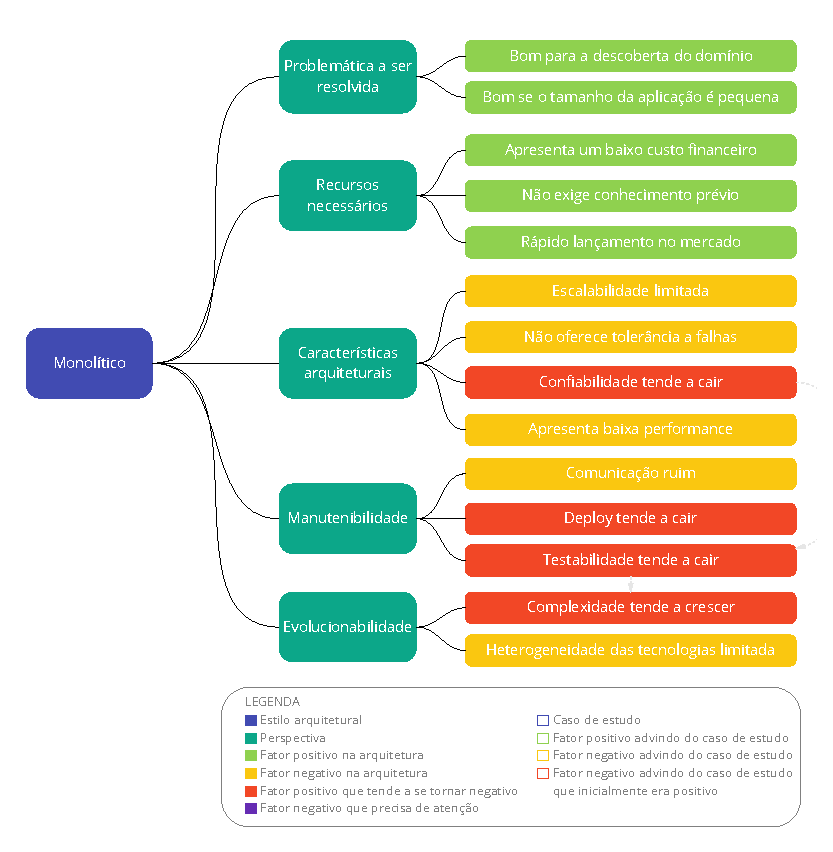
\includegraphics[keepaspectratio=true,scale=1]{figuras/sintese-monolitico.eps}
  \caption{Mapa mental do processo de síntese realizado sobre a arquitetura monolítica\label{fig:SinteseMono}}
\end{figure}
\newpage

\section{Síntese da arquitetura de microsserviços}

\begin{quadro}
    \caption{Arquitetura de microsserviços - síntese sobre o domínio do problema\label{microsservicos:sintese-dominio}}
    \begin{tabularx}{\linewidth}{ | p{5cm} | X | }
    \hline
    \textbf{A escolha de uma}       & arquitetura de microsserviços \\ \hline
    \textbf{sob a perspectiva}      & da problemática a ser resolvida \\ \hline
    \textbf{mediante o aspecto}     & de domínio sobre o problema \\ \hline
    \textbf{gera um impacto}        & de necessidade de domínio sobre o contexto\\ \hline
    \textbf{devido à }              & definição dos limites que impacta toda a arquitetura \\ \hline
    % \textbf{contudo}                & \\ \hline
    % \textbf{consciente de que este aspecto tende a }          & \\ \hline
    \textbf{com base na}            & \autoref{Perspectivas:Problematica} \\ \hline
    \end{tabularx}
\end{quadro}

\begin{quadro}
    \caption{Arquitetura de microsserviços - síntese sobre o tamanho da aplicação\label{microsservicos:sintese-tamanho}}
    \begin{tabularx}{\linewidth}{ | p{5cm} | X | }
    \hline
    \textbf{A escolha de uma}       & arquitetura de microsserviços \\ \hline
    \textbf{sob a perspectiva}      & da problemática a ser resolvida \\ \hline
    \textbf{mediante o aspecto}     & do tamanho planejado para a aplicação \\ \hline
    \textbf{gera um impacto}        & de custo muito alto para aplicações pequenas \\ \hline
    \textbf{devido ao}              & custo muito alto de implementação e manutenção\\ \hline
    % \textbf{contudo}                & \\ \hline
    % \textbf{consciente de que este aspecto tende a} & \\ \hline
    \textbf{com base na}            & \autoref{Perspectivas:Problematica} \\ \hline
    \end{tabularx}
\end{quadro}

\begin{quadro}
    \caption{Arquitetura de microsserviços - síntese sobre os recursos financeiros\label{microsservicos:sintese-financeiros}}
    \begin{tabularx}{\linewidth}{ | p{5cm} | X | }
    \hline
    \textbf{A escolha de uma}       & arquitetura de microsserviços \\ \hline
    \textbf{sob a perspectiva}      & recursos necessários \\ \hline
    \textbf{mediante o aspecto}     & de recursos financeiros \\ \hline
    \textbf{gera um impacto}        & alto custo \\ \hline
    \textbf{devido à }              & necessidade de mão de obra especializada, monitoramento, replicação...\\ \hline
    % \textbf{contudo}                & \\ \hline
    % \textbf{consciente de que este aspecto tende a} & \\ \hline
    \textbf{com base na}            & \autoref{Perspectivas:recursosFinanceiros} \\ \hline
    \end{tabularx}
\end{quadro}

\begin{quadro}
    \caption{Arquitetura de microsserviços - síntese sobre os recursos humanos\label{microsservicos:sintese-humanos}}
    \begin{tabularx}{\linewidth}{ | p{5cm} | X | }
    \hline
    \textbf{A escolha de uma}       & arquitetura de microsserviços \\ \hline
    \textbf{sob a perspectiva}      & recursos necessários \\ \hline
    \textbf{mediante o aspecto}     & de recursos humanos \\ \hline
    \textbf{gera um impacto}        & necessita de expertise sobre as tecnologias \\ \hline
    \textbf{devido à }              & complexidade da arquitetura \\ \hline
    % \textbf{contudo}                & \\ \hline
    % \textbf{consciente de que este aspecto tende a} & \\ \hline
    \textbf{com base na}            & \autoref{Perspectivas:recursosHumanos} \\ \hline
    \end{tabularx}
\end{quadro}

\begin{quadro}
    \caption{Arquitetura de microsserviços - síntese sobre esforço e tempo inicial\label{microsservicos:sintese-esforco}}
    \begin{tabularx}{\linewidth}{ | p{5cm} | X | }
    \hline
    \textbf{A escolha de uma}       & arquitetura de microsserviços \\ \hline
    \textbf{sob a perspectiva}      & recursos necessários \\ \hline
    \textbf{mediante o aspecto}     & esforço e tempo inicial \\ \hline
    \textbf{gera um impacto}        & alto esforço inicial e demorado lançamento no mercado \\ \hline
    \textbf{devido à }              & complexidade da arquitetura e a necessidade de automatizar todos os processos operacionais \\ \hline
    % \textbf{contudo}                & \\ \hline
    % \textbf{consciente de que este aspecto tende a} & \\ \hline
    \textbf{com base na}            & \autoref{effortsAndTime} \\ \hline
    \end{tabularx}
\end{quadro}

\begin{quadro}
    \caption{Arquitetura de microsserviços - síntese sobre escalabilidade\label{microsservicos:sintese-escalabilidade}}
    \begin{tabularx}{\linewidth}{ | p{5cm} | X | }
    \hline
    \textbf{A escolha de uma}       & arquitetura de microsserviços \\ \hline
    \textbf{sob a perspectiva}      & de características arquiteturais \\ \hline
    \textbf{mediante o aspecto}     & da escalabilidade \\ \hline
    \textbf{gera um impacto}        & de ser altamente escalável \\ \hline
    \textbf{devido à }              & alta modularidade e automatização dos processos \\ \hline
    % \textbf{contudo}                & \\ \hline
    % \textbf{consciente de que este aspecto tende a} & \\ \hline
    \textbf{com base na}            & \autoref{pers:escalabilidade} \\ \hline
    \end{tabularx}
\end{quadro}

\begin{quadro}
    \caption{Arquitetura de microsserviços - síntese sobre tolerância a falhas\label{microsservicos:sintese-tolerancia}}
    \begin{tabularx}{\linewidth}{ | p{5cm} | X | }
    \hline
    \textbf{A escolha de uma}       & arquitetura de microsserviços \\ \hline
    \textbf{sob a perspectiva}      & de características arquiteturais \\ \hline
    \textbf{mediante o aspecto}     & de tolerância a falhas \\ \hline
    \textbf{gera um impacto}        & alta tolerância \\ \hline
    \textbf{devido à }              & presença de vários pontos de falha, comprometendo apenas parcialmente a aplicação\\ \hline
    \textbf{contudo}                & é preciso lidar com a escalabilidade da rede \\ \hline
    % \textbf{consciente de que este aspecto tende a} & \\ \hline
    \textbf{com base na}            & \autoref{pers:tolerancia} \\ \hline
    \end{tabularx}
\end{quadro}

\begin{quadro}
    \caption{Arquitetura de microsserviços - síntese sobre confiabilidade\label{microsservicos:sintese-confiabilidade}}
    \begin{tabularx}{\linewidth}{ | p{5cm} | X | }
    \hline
    \textbf{A escolha de uma}       & arquitetura de microsserviços \\ \hline
    \textbf{sob a perspectiva}      & de características arquiteturais \\ \hline
    \textbf{mediante o aspecto}     & de confiabilidade do sistema \\ \hline
    \textbf{gera um impacto}        & alta confiabilidade \\ \hline
    % \textbf{devido à }              & \\ \hline
    \textbf{contudo}                & é preciso lidar com eventuais inconsistências e escalabilidade da rede\\ \hline
    % \textbf{consciente de que este aspecto tende a} & decair a medida que a base de código aumenta \\ \hline
    \textbf{com base na}            & \autoref{pers:confiabilidade} \\ \hline
    \end{tabularx}
\end{quadro}

\begin{quadro}
    \caption{Arquitetura de microsserviços - síntese sobre performance\label{microsservicos:sintese-performance}}
    \begin{tabularx}{\linewidth}{ | p{5cm} | X | }
    \hline
    \textbf{A escolha de uma}       & arquitetura de microsserviços \\ \hline
    \textbf{sob a perspectiva}      & de características arquiteturais \\ \hline
    \textbf{mediante o aspecto}     & de performance do sistema \\ \hline
    \textbf{gera um impacto}        & baixa performance \\ \hline
    \textbf{devido à }              & dependência da rede e da adição de várias camadas de segurança
        na comunicação entre os serviços \\ \hline
    % \textbf{contudo}                & \\ \hline
    % \textbf{consciente de que este aspecto tende a} & \\ \hline
    \textbf{com base na}            & \autoref{pers:performance} \\ \hline
    \end{tabularx}
\end{quadro}

\begin{quadro}
    \caption{Arquitetura de microsserviços - síntese sobre o processo de \textit{deploy}\label{microsservicos:sintese-deploy}}
    \begin{tabularx}{\linewidth}{ | p{5cm} | X | }
    \hline
    \textbf{A escolha de uma}       & arquitetura de microsserviços \\ \hline
    \textbf{sob a perspectiva}      & de manutenibilidade \\ \hline
    \textbf{mediante o aspecto}     & de implantação do sistema \\ \hline
    \textbf{gera um impacto}        & de fácil e rápida de implantação \\ \hline
    \textbf{devido}                 & aos processos automatizados \\ \hline
    \textbf{contudo}                & é preciso automatizar os processos operacionais \\ \hline
    % \textbf{consciente de que este aspecto tende a} & decair a medida que a base de código fica maior \\ \hline
    \textbf{com base na}            & \autoref{pers:deploy} \\ \hline
    \end{tabularx}
\end{quadro}

\begin{quadro}
    \caption{Arquitetura de microsserviços - síntese da testabilidade\label{microsservicos:sintese-testabilidade}}
    \begin{tabularx}{\linewidth}{ | p{5cm} | X | }
    \hline
    \textbf{A escolha de uma}       & arquitetura de microsserviços \\ \hline
    \textbf{sob a perspectiva}      & de manutenibilidade \\ \hline
    \textbf{mediante o aspecto}     & de testabilidade do sistema \\ \hline
    \textbf{gera um impacto}        & fácil de uma perspectiva local e difícil de uma perspectiva global \\ \hline
    \textbf{devido à }              & modularidade local e a complexidade global respectivamente \\ \hline
    % \textbf{contudo}                & é preciso lidar com a crescente complexidade\\ \hline
    % \textbf{consciente de que este aspecto tende a} & decair a medida que a complexidade do sistema aumenta \\ \hline
    \textbf{com base na}            & \autoref{testabilidade} \\ \hline
    \end{tabularx}
\end{quadro}

\begin{quadro}
    \caption{Arquitetura de microsserviços - síntese da comunicação\label{microsservicos:sintese-comunicacao}}
    \begin{tabularx}{\linewidth}{ | p{5cm} | X | }
    \hline
    \textbf{A escolha de uma}       & arquitetura de microsserviços \\ \hline
    \textbf{sob a perspectiva}      & de manutenibilidade \\ \hline
    \textbf{mediante o aspecto}     & de comunicação entre os times \\ \hline
    \textbf{gera um impacto}        & positivo \\ \hline
    \textbf{devido aos}             & times multifuncionais \\ \hline
    % \textbf{contudo}                & é preciso lidar com a comunicação entre diferentes áreas\\ \hline
    % \textbf{consciente de que este aspecto tende a} & decair a medida que a complexidade do sistema aumenta \\ \hline
    \textbf{com base na}            & \autoref{pers:comunicacao} \\ \hline
    \end{tabularx}
\end{quadro}

\begin{quadro}
    \caption{Arquitetura de microsserviços - síntese da heterogeneidade das tecnologias\label{microsservicos:sintese-heterogeneidade}}
    \begin{tabularx}{\linewidth}{ | p{5cm} | X | }
    \hline
    \textbf{A escolha de uma}       & arquitetura de microsserviços \\ \hline
    \textbf{sob a perspectiva}      & de evolucionabilidade \\ \hline
    \textbf{mediante o aspecto}     & de heterogeneidade das tecnologias \\ \hline
    \textbf{gera um impacto}        & de alta heterogeneidade \\ \hline
    \textbf{devido ao}              & modelo arquitetural com baixo acoplamento \\ \hline
    % \textbf{contudo}                & é preciso lidar com a comunicação entre diferentes áreas\\ \hline
    % \textbf{consciente de que este aspecto tende a} & decair a medida que a complexidade do sistema aumenta \\ \hline
    \textbf{com base na}            & \autoref{pers:heterogeneidade} \\ \hline
    \end{tabularx}
\end{quadro}

\begin{quadro}
    \caption{Arquitetura de microsserviços - síntese sobre complexidade do sistema\label{microsservicos:sintese-complexidade}}
    \begin{tabularx}{\linewidth}{ | p{5cm} | X | }
    \hline
    \textbf{A escolha de uma}       & arquitetura de microsserviços \\ \hline
    \textbf{sob a perspectiva}      & de evolucionabilidade \\ \hline
    \textbf{mediante o aspecto}     & da complexidade do sistema \\ \hline
    \textbf{gera um impacto}        & de baixa complexidade de uma perspectiva local e alta
        complexidade de uma perspectiva global\\ \hline
    \textbf{devido ao}              & característica distribuída da arquitetura \\ \hline
    % \textbf{contudo}                & é preciso lidar com o acoplamento do código \\ \hline
    % \textbf{consciente de que este aspecto tende a} & crescer a medida que ao crescimento da base de código\\ \hline
    \textbf{com base na}            & \autoref{pers:heterogeneidade} \\ \hline
    \end{tabularx}
\end{quadro}

\newpage

A \autoref{fig:SinteseMicro} visa ilustrar um resumo dos pontos destacados com base na síntese
elaborada a partir do referêncial teórico. Nela podemos observar de verde os fatores positivos da
arquitetura, de amarelo os fatores negativos e de roxo os fatores que em geral são positivos na
arquitetura mas que exigem que o time de desenvolvimento lide com algum fator adverso. Por exemplo,
o \textit{deploy} é apontado como um fator positivo dentro da arquitetura de microsserviços, visto
que é fácil e rápido atualizar um serviço, contudo existe o fator adverso de que todo o processo
deve estar automatizado, caso a equipe não automatize esse processo, provavelmente eles terão algum
problema pra lidar com o \textit{deploy} dentro dessa arquitetura.

\begin{figure}[h]
  \centering
  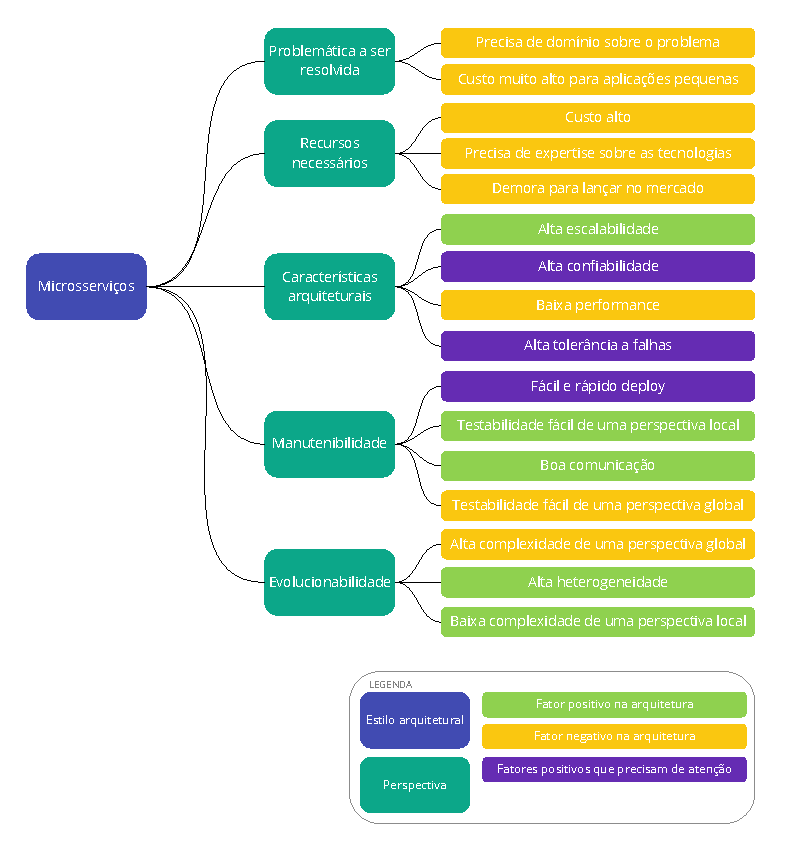
\includegraphics[keepaspectratio=true,scale=1]{figuras/sintese-microsservicos.eps}
  \caption{Mapa mental do processo de síntese realizado sobre a arquitetura de microsserviços\label{fig:SinteseMicro}}
\end{figure}
